\documentclass{article}

\usepackage{amsmath, graphicx}

\graphicspath{ {./images/} }

\title{Ch. 27 Solutions}
\author{Principles of Macroeconomics}
\date{today}

\begin{document}

\maketitle

\section*{Quick Quiz}

\begin{enumerate}

\item (d) -- A bond is essentially a loan, and a stock is an ownership share, so Clarke is a bondholder, and Jimmy is a stockholder.

\item (d) -- The higher the credit risk, the higher the interest rate.

\item (b) -- Mutual funds tend to whole multiple assets, so they provide diversification.

\item (d) -- If tax revenue is more than government spending, then public saving ($T - G$) is positive. If consumption is greater than after tax income, then private saving, ($Y - T - C$) is negative.

\item (c) --
	\begin{gather*}
	S_{Nat} = S_{Priv} + S_{Pub} \\
	S_{Nat} = I = \$250 \\
	S_{Pub} = T - G = \$150 -\$200 = -\$50 \\
	\$250 = S_{Priv} + -\$50 \\
	\$300 = S_{Priv}
	\end{gather*}

\item (b) -- An increase in saving is an increase in supply. When the supply of loanable funds shifts right, the interest rate falls.

	\begin{center}
	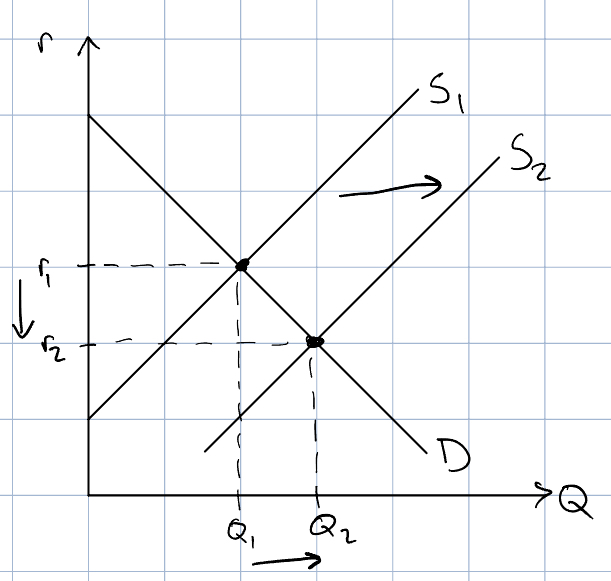
\includegraphics[width = 0.5\textwidth]{qq6}
	\end{center}

\item (c) -- If businesses expect capital to be more profitable, they will want to invest more. That increases their demand for loanable funds, so demand shifts right, and the interest rate rises. 

	\begin{center}
	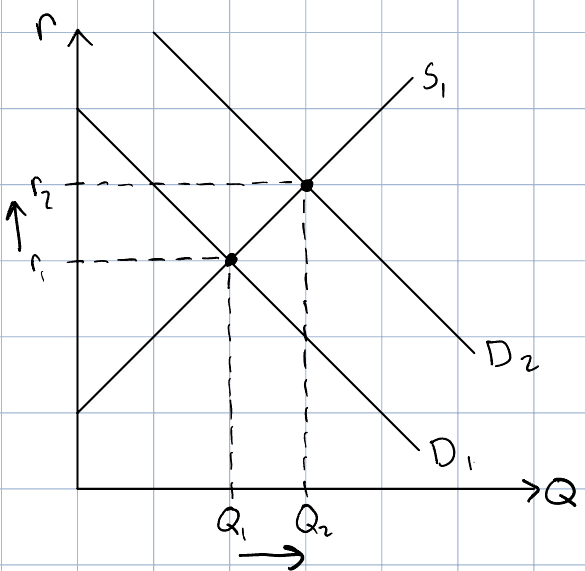
\includegraphics[width = 0.5\textwidth]{qq7}
	\end{center}

\item (b) -- An increase in the government budget deficit decreases public saving. That shifts the supply of loanable funds to the left, increases the interest rate, and decreases the equilibrium quantity of investment. That's why we say the government ``crowds out" investment when it runs a deficit.

	\begin{center}
	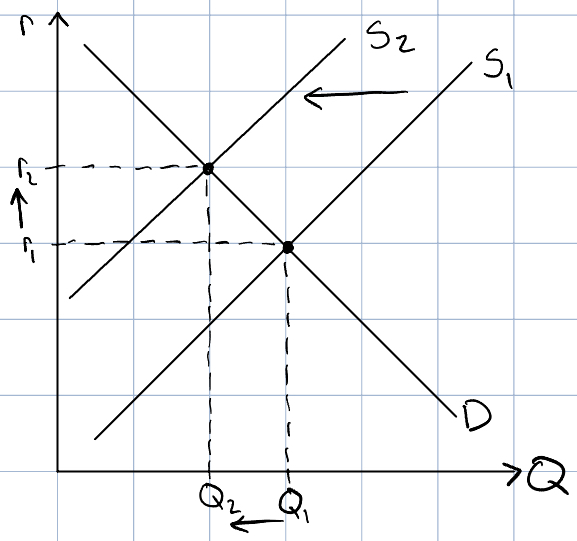
\includegraphics[width = 0.5\textwidth]{qfr6}
	\end{center}

\item (a) -- See Figure 6 in 27.3.d. 

\end{enumerate}



\section*{Questions for Review}

\begin{enumerate}

\item The role of the financial system is to channel money from savers to investors.

One financial market is the bond market where people essentially buy IOUs from firms and governments. Another is the stock market where people buy ownership shares of firms. 

One financial intermediary is a bank which takes deposits from savers and uses them to make loans to investors. Another is a mutual fund which pools money from savers and uses the proceeds to buy a portfolio of stocks and bonds. 

\item Diversification allows investors to decrease the risk of their portfolio by holding a small share of a lot of companies. Mutual funds make diversification easier because investors can buy a share of a mutual fund and own a small part of the mutual fund's entire portfolio.

\item National saving is the total income left over after consumption and government purchases: $S_{Nat} = Y - C - G$ \\
	Private saving is the total income left over after consumption and taxes: $S_{Priv} = Y - T - C$ \\
	Public saving is the tax revenue left over after government purchases: $S_{Pub} = T - G$ \\
	National saving is the sum of private saving and public saving: \\ $S_{Nat} = S_{Priv} + S_{Pub}$
	
\item Investment is spending on capital goods. In a closed economy, investment equals national saving: $I = S_{Nat}$

\item A decrease in the tax on interest earnings will make saving more lucrative. That will incentivize households to save more, so private saving increases. Importantly, we have to assume that the increase in private saving is larger than the decrease in public saving due to the decrease in tax revenue.

In the market for loanable funds, an increase in saving shifts supply right, drives the interest rate down, and increases the quantity of investment in the economy.

	\begin{center}
	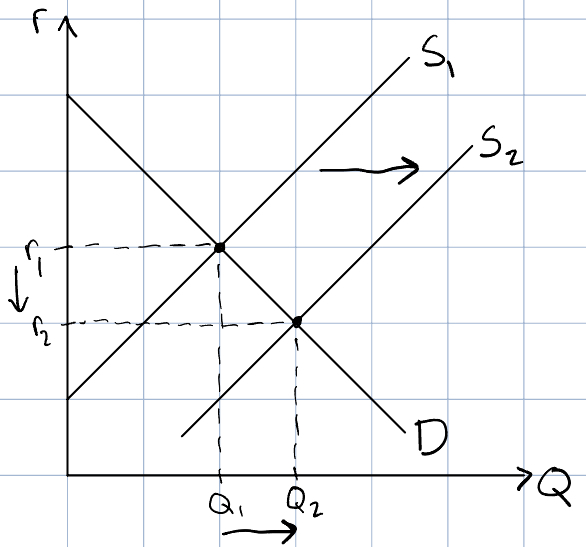
\includegraphics[width = 0.5\textwidth]{qfr5}
	\end{center}
	
\item A government budget deficit occurs when the government spends more than it collects in tax revenue. It decreases public saving which shifts the supply of loanable funds to the left. That in turn increases the interest rate and decreases the quantity of investment in the economy.

	\begin{center}
	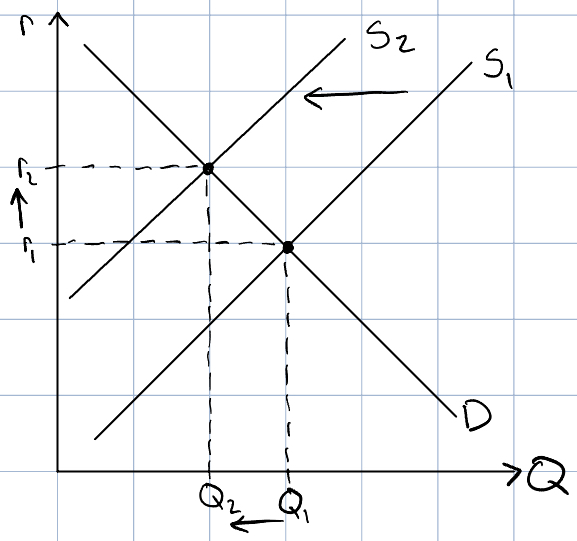
\includegraphics[width = 0.5\textwidth]{qfr6}
	\end{center}
Lower investment leads to slower growth in the capital stock. Lower growth in the capital stock leads to slower economic growth.

\end{enumerate}



\section*{Problems \& Applications}

\begin{enumerate}

\item

	\begin{enumerate}
	
	\item Eastern European government  -- Lending to the U.S. government is probably less of a credit risk than lending to the Eastern European government because the economy is probably stronger and the government is probably more politically stable.
	
	\item 2050 -- A longer term leaves more time for the corporation to fall on hard times and potentially default, so longer term bonds pose a bigger credit risk.
	
	\item The software company -- The software company is less established and less well-known than Coca-Cola, so investors probably view it as a greater credit risk.
	
	\item Federal -- Interest earned on state bonds is exempt from the federal income tax, so state governments don't have to pay as much interest as the federal government.
	
	\end{enumerate}
	
\item Companies encourage workers to own stock in the firm because it gives them an ownership interest in the firm. That means they receive a portion of the firms’ future profits, so they’re more invested in their company’s success. That gives them a greater incentive to do high quality work. 

Employees might not want to hold stock in the company where they work because then they are highly dependent on the success of a single company. Both their wages and their savings depend on the success of that company. That’s riskier than diversifying their savings across a number of companies where they don’t work.

\item Saving is money not spent on consumption or government purchases. Investment is money spent on capital.

	\begin{enumerate}
	
	\item Investment -- New housing is considered capital.
	
	\item Saving -- A stock isn't capital.
	
	\item Saving -- The deposit is money left over after consumption and taxes. Here, taxes are relevant because individuals contribute to private saving, and private saving is income left over after consumption and taxes.
	
	\item Investment -- A car for a delivery business is a capital good.
	
	\end{enumerate}
	
\item \begin{gather*}
	S_{Nat} = S_{Pub} + S_{Priv} = 0.5 + 0.2 = \$0.7 \text{ trillion} \\
	I = S_{Nat} = \$0.7 \text{ trillion} \\
	S_{Pub} = T - G \implies G = T - S_{Pub} = 1.5 - 0.2 = \$1.3 \text{ trillion} \\
	Y = C + I + G \implies C = Y - I - G = 8 - 0.7 - 1.3 = \$ 6 \text{ trillion}
	\end{gather*}
	
\item \begin{gather*}
	S_{Priv} = Y - T - C = 10,000 - 1,500 - 6,000 = 2,500 \\
	S_{Pub} = T - G = 1,500 - 1,700 = -200 \\
	S_{Nat} = S_{Priv} + S_{Pub} = 2,500 - 200 = 2,300 \\
	I = S_{Nat} = 2,300
	\end{gather*}
	\begin{align*}
	I &= 3,300 - 100r \\
	2,300 &= 3,300 - 100r \\
	100r &= 1,000 \\
	r &= 10\%
	\end{align*}
	
\item

	\begin{enumerate}
	
	\item Higher interest rates make it more expensive for Intel to borrow money for the factory. That makes them less likely to build the factory. 
	
	\item It would. Higher interest rates make it more lucrative for Intel to save its money rather than spend it. That makes them more likely to save and less likely to build the factory.
	
	\end{enumerate}
	
\item

	\begin{enumerate}
	
	\item Harry: \$1,000(1.05) = \$1,050 \\
		Ron: \$1,000(1.08) = \$1,080 \\
		Hermione \$1,000(1.20) = \$1,200
		
	\item If the rate of return on their investment is greater than $r$, then they would borrow because they would make more money on the investment than they would spend on interest. If the rate of return on their investment is lower than $r$, then they would lend because they would make more money from interest than they would on the investment.
	
	\item At 7\%, Ron and Hermione would both want to borrow, so the quantity of loanable funds demanded would be \[ \$1,000 + \$1,000 = \$2,000. \] Harry would want to save, so the quantity of loanable funds supplied would be \$1,000. \\
	At 10\%, Hermione would want to borrow, so the quantity of loanable funds demanded would be \$1,000. Harry and Ron would both want to save, so the quantity of loanable funds supplied would be \[\$1,000 + \$1,000 = \$2,000. \]
	
	\item At an interest rate of 8\%, the market for loanable funds would be at equilibrium. Harry would want to lend \$1,000, and Hermione would want to borrow \$1,000. Ron would be indifferent between borrowing and lending, so he would likely do neither and just invest his own money. 
	
	\item Harry: \$1,000(1.08) = \$1,080 \\
		Ron: \$1,000(1.08) = \$1,080 \\
		Hermione: \$2,000(1.20) - \$1,000(1.08) = \$2,400 - \$1,080 = \$1,320
		
		Harry and Hermione both benefit from loanable funds market because they make more money than they would without it. Ron is just as well off as he would be  without it, so no one's worse off.
	
	\end{enumerate}
	
\item

	\begin{enumerate}
	
	\item If the government borrows more next year, then the budget deficit will increase. That will decrease public saving and therefore national saving. The supply of national saving will shift left, so the interest rate will rise.
	
	\begin{center}
	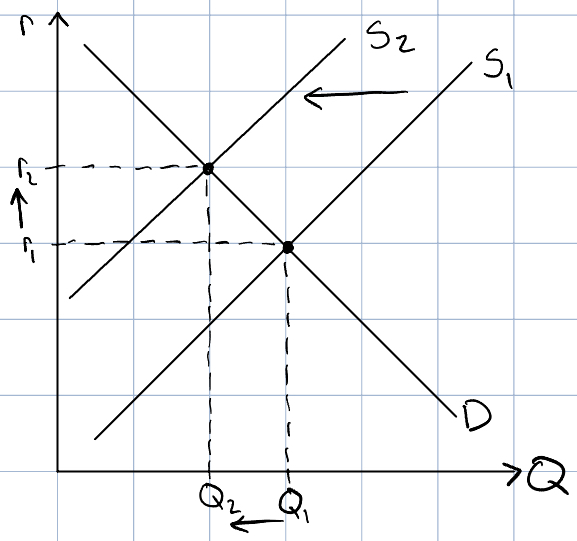
\includegraphics[width = 0.5\textwidth]{qfr6}
	\end{center}
	
	\item When the budget deficit increases by \$20 billion, public saving decreases by \$20 billion. As a result, the supply of loanable funds shifts left by \$20 billion, and the quantity of national saving and investment decreases. National saving and investment decrease by less than the \$20 billion shift in supply because the interest rate increases. When the interest rate increases, it incentivizes households to save more, so private saving increases and offsets some of the \$20 billion decrease in public saving. 
	
	\begin{center}
	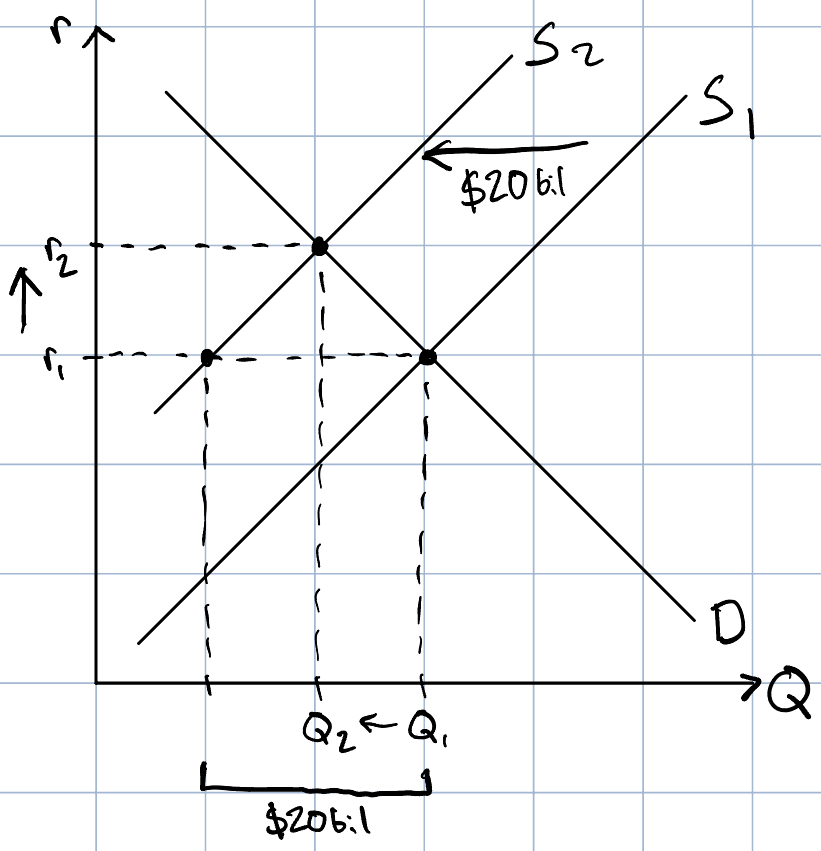
\includegraphics[width = 0.5\textwidth]{paa8b}
	\end{center}
	
	\item If the supply of loanable funds is more elastic, the decrease in public saving will be unaffected; the decrease in national saving and investment will be smaller, and the increase in private saving will be larger.
	
	\begin{center}
	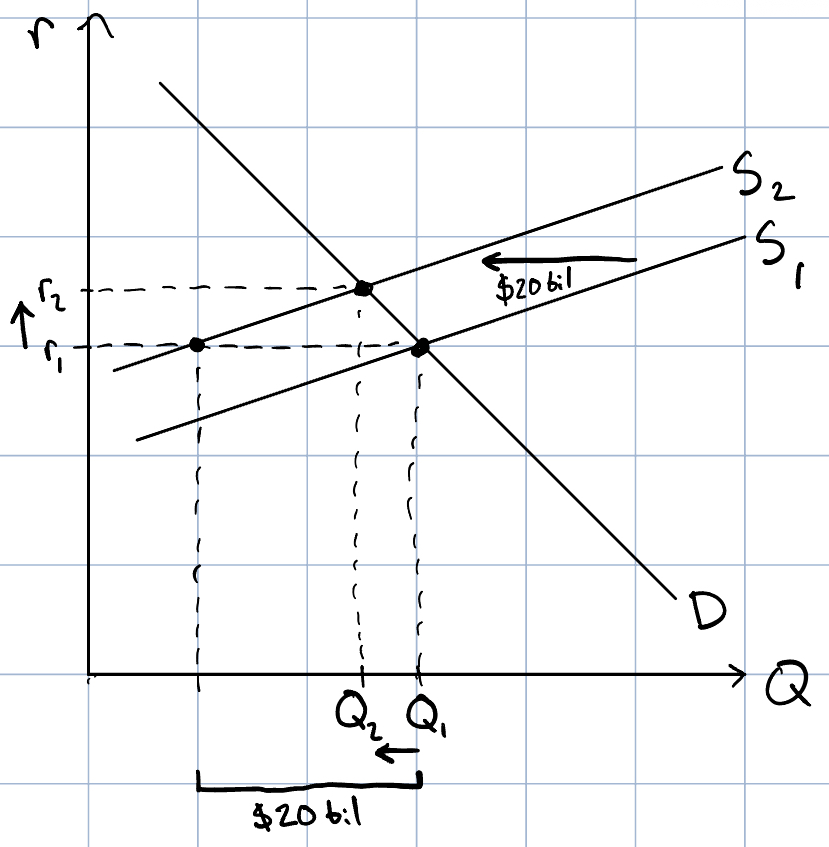
\includegraphics[width = 0.5\textwidth]{paa8c}
	\end{center}
	
	\item If the demand for loanable funds is more elastic, the decrease in public saving will be unaffected; the decrease in national saving and investment will be larger, and the increase in private saving will be smaller.
	
	\begin{center}
	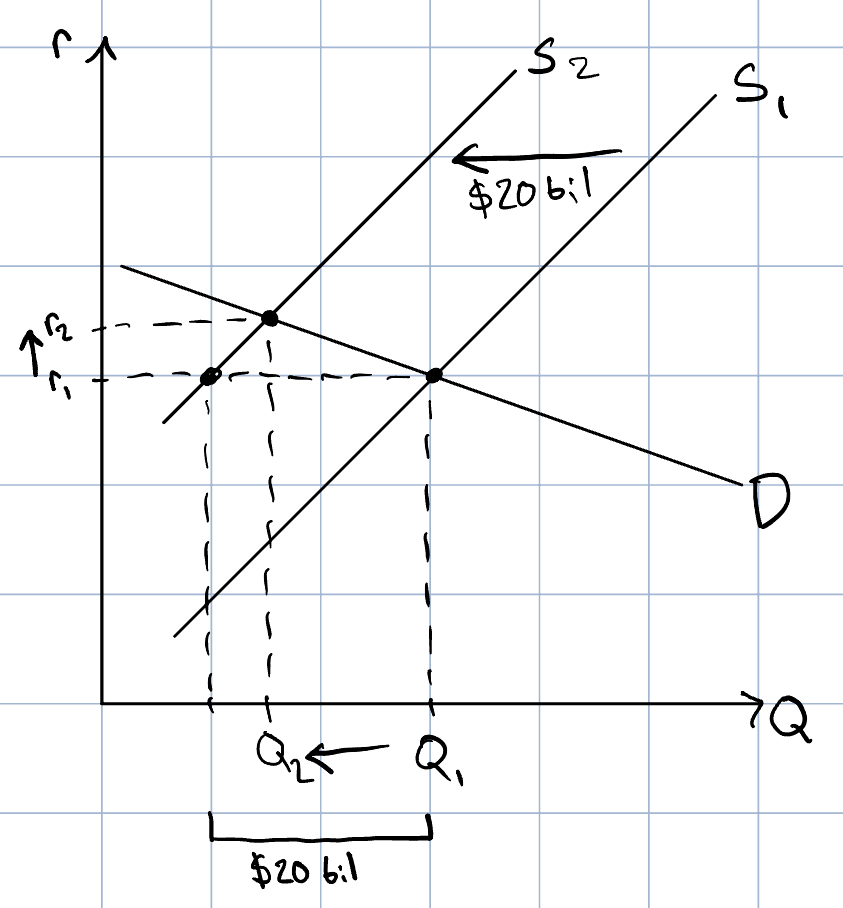
\includegraphics[width = 0.5\textwidth]{paa8d}
	\end{center}
	
	\item If households expected higher taxes in the future, they would save more today in order to pay those taxes in the future. Therefore, private saving would increase, and the supply of loanable funds would shift less than \$20 billion dollars to the left. That means. private saving would increase more, national saving would decrease less, investment would decrease less, and the interest rate would increase less than they did in parts (a) and (b). Public saving would still decrease by \$20 billion.
	
	\begin{center}
	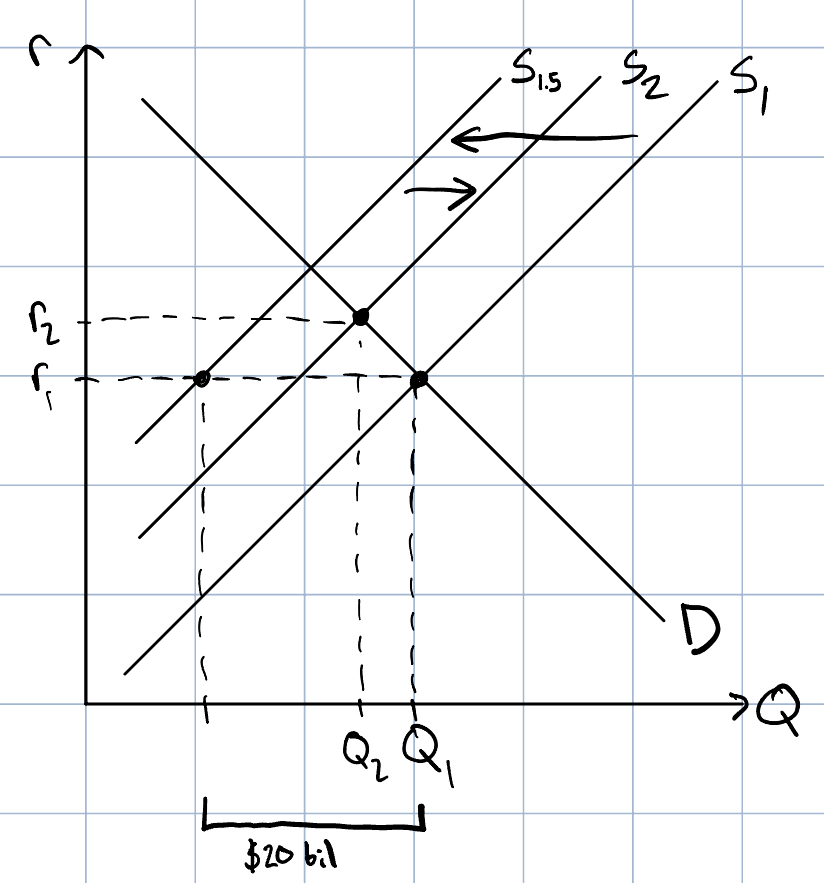
\includegraphics[width = 0.5\textwidth]{paa8e}
	\end{center}
	
	\end{enumerate}
	
\item

	\begin{enumerate}
	
	\item If government spending stays the same, a tax cut will increase the budget deficit. To cut taxes and reduce the deficit, the government would have to cut spending more than it cuts taxes.
	
	\item We would need to know how much private saving increases in response to a tax cut. A decrease in the government budget deficit increases public saving by the exact amount that the budget deficit decreases. It's less clear how responsive households are to tax cuts. Whichever policy increased saving more would increase investment more.
	
	\end{enumerate}

\end{enumerate}

\end{document}